\chapter{Моделирование TGE и TGF
}\label{ch:thunderstorm}

\section{Обзор экспериментальных результатов
}\label{sec:thunderstorm/review-exp}

\section{Обзор существующих моделей}\label{sec:thunderstorm/review-mod}

\subsection{Пробой на убегающих электронах}
%
Пробой на убегающих электронах (ПУЭ) --- модель развития лавины релятивистских (с энергией 0.1 --- 10 МэВ) электронов в постоянном электрическом поле предложенная А.~В.~Гуревичем~\cite{gurevich1992runaway,Gurevich2001ufn}. Качественно идея модели проста: пусть электрон ускоряется за счет электрического поля и тормозится за счет взаимодействия со средой, если он получает от поля больше энергии чем теряет, то у него появляется избыток энергии, который может быть потрачен на рождение нового электрона. Такие электроны будем называть убегающими. Если пренебречь всеми процессами кроме ионизационных потерь и радиационных потерь, то \todo{график} показывает условия генерации лавины убегающих электронов в однородном поле. Энергию при которой электрон в среднем на единице длинны приобретает энергии больше чем теряет мы будем называть критической.

\begin{figure}[t]
    \begin{center}
        \begin{minipage}[h]{0.49\linewidth}
            \center{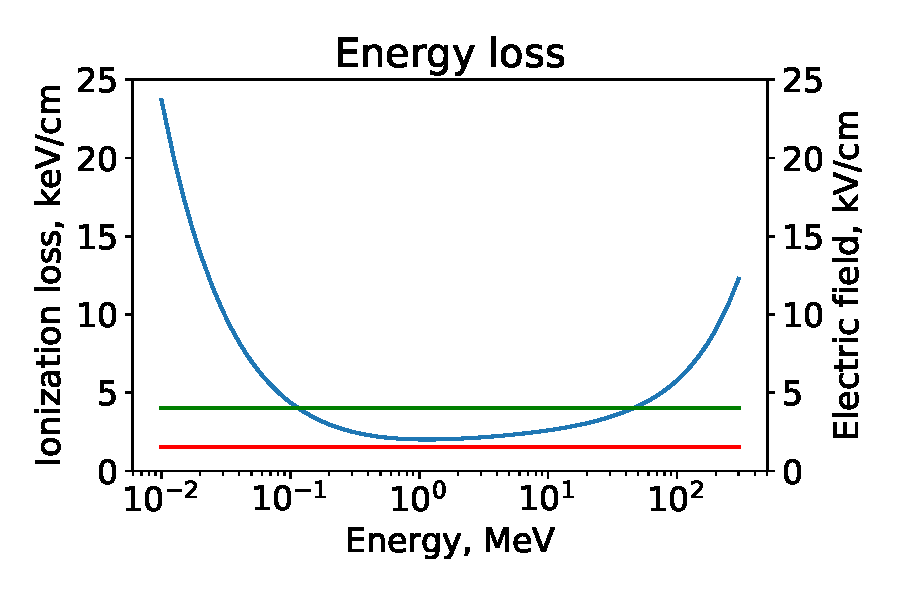
\includegraphics[width=\linewidth]{thunderstorm/01_Gurevich.pdf} \\ а)}
        \end{minipage}
        \hfill
        \begin{minipage}[h]{0.49\linewidth}
            \center{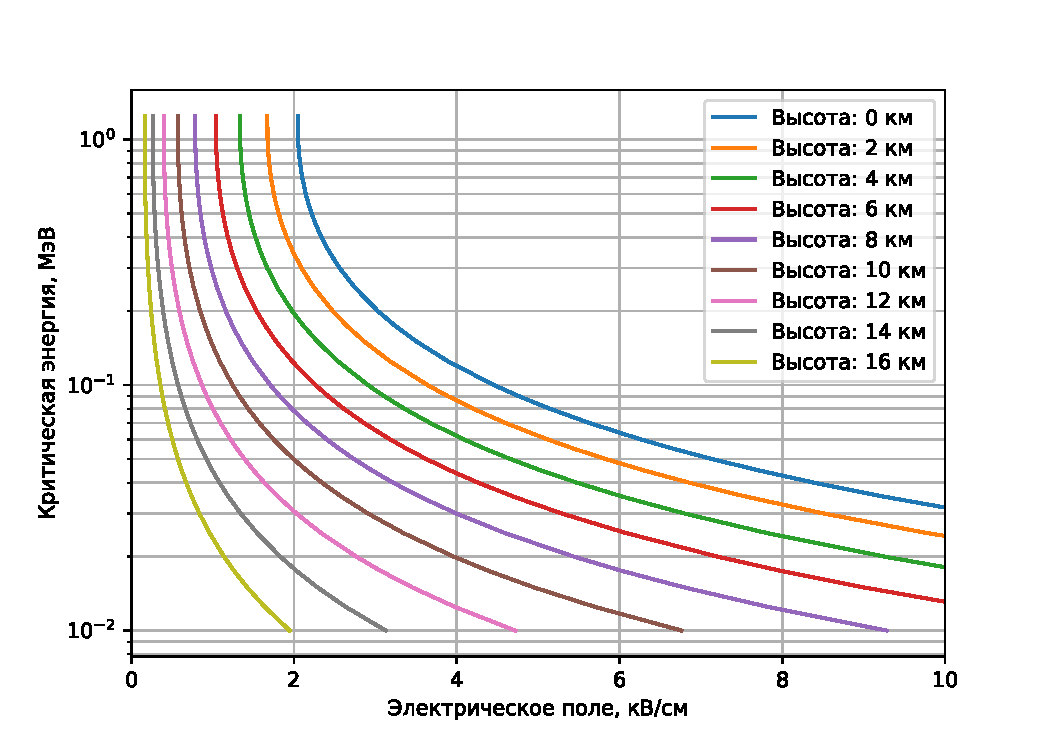
\includegraphics[width=\linewidth]{thunderstorm/02_CriticalEnergy.pdf}   \\ б)}
        \end{minipage}
        \caption{а) Ионизационные потери электронов в воздухе при нормальных условиях. б) Зависимость критической энергии от поля для различных высот.}
    \end{center}
    \label{thunder:gurevich}
\end{figure}

\subsection{Модели атмосферы}
Для установления значения плотности воздуха на разных высотах в моделировании используется международная стандартная модель атмосферы (ISA)


\section{Моделирование RREA, сравнение с результатами Гуревича, Орешкина.}\label{sec:thunderstorm/rrea}



\section{Расчет коэффициента обратной связи, сравнение с результатами Дваера}\label{sec:thunderstorm/rdfm}
\section{Reactor like TGE-model}\label{sec:thunderstorm/reactor}

Общим недостатком рассмотренных выше моделей является упрощенная модель электрического поля: оно считается однородным по величине и направлению, что очевидно не так и в полу должны присутствовать разного рода неоднородности, вызванные как краевыми эффектами, так и возникновением сложных конфигураций зарядов. Точное моделирование и анализ динамики лавин убегающих электронов представляет собой сложную задачу, поэтому рассмотрим упрощенную модель что бы оценить потенциальные результаты, которые могут принести исследования в данном направлении. 

Чем ситуация в неоднородном по направлению поле отличается от развития лавин в однородном поле? Когда поле однородно то если гамма-кванты рождают новые затравочные электроны, то лавины от этих электронов будут направлены в том же направлении что и  первая лавина, но при этом их вершина будет смещена к  краю облака, что будет постепенно приводить к затуханию (как показано в предыдущих главах). Если же поле неоднородно по направлению, то направление новых лавин зависит от локальной конфигурации поля и таким образом может возникнуть ситуация изображенная на рисунке --- гамма-кванты от первичной лавины "зажигают" новые локальные ускоряющие ячейки, которые генерирует гамма кванты с угловым распределение значительно повернутым относительно углового распределения исходной лавины, что способствует более равномерному распределению новых затравочных электронов по облаку и как следствие  самоподдерживающей генерации лавин убегающих электронов.
Что бы смоделировать этот процесс, мы рассмотрим такую модель:
\begin{itemize}
    \item  Электрннная лавина не расмтриается детально, аработает только как ускоряющая ячейка которая 
\end{itemize}
\begin{figure}
    \centering
    \begin{overpic}[scale=.5]{thunderstorm/rltge/electric_streams.pdf}
        \put(15,53){\includegraphics[scale=.015]{thunderstorm/rltge/cell.pdf}}
        \put(20,69){\text{Ускоряющая ячейка}}
        \put(10,10){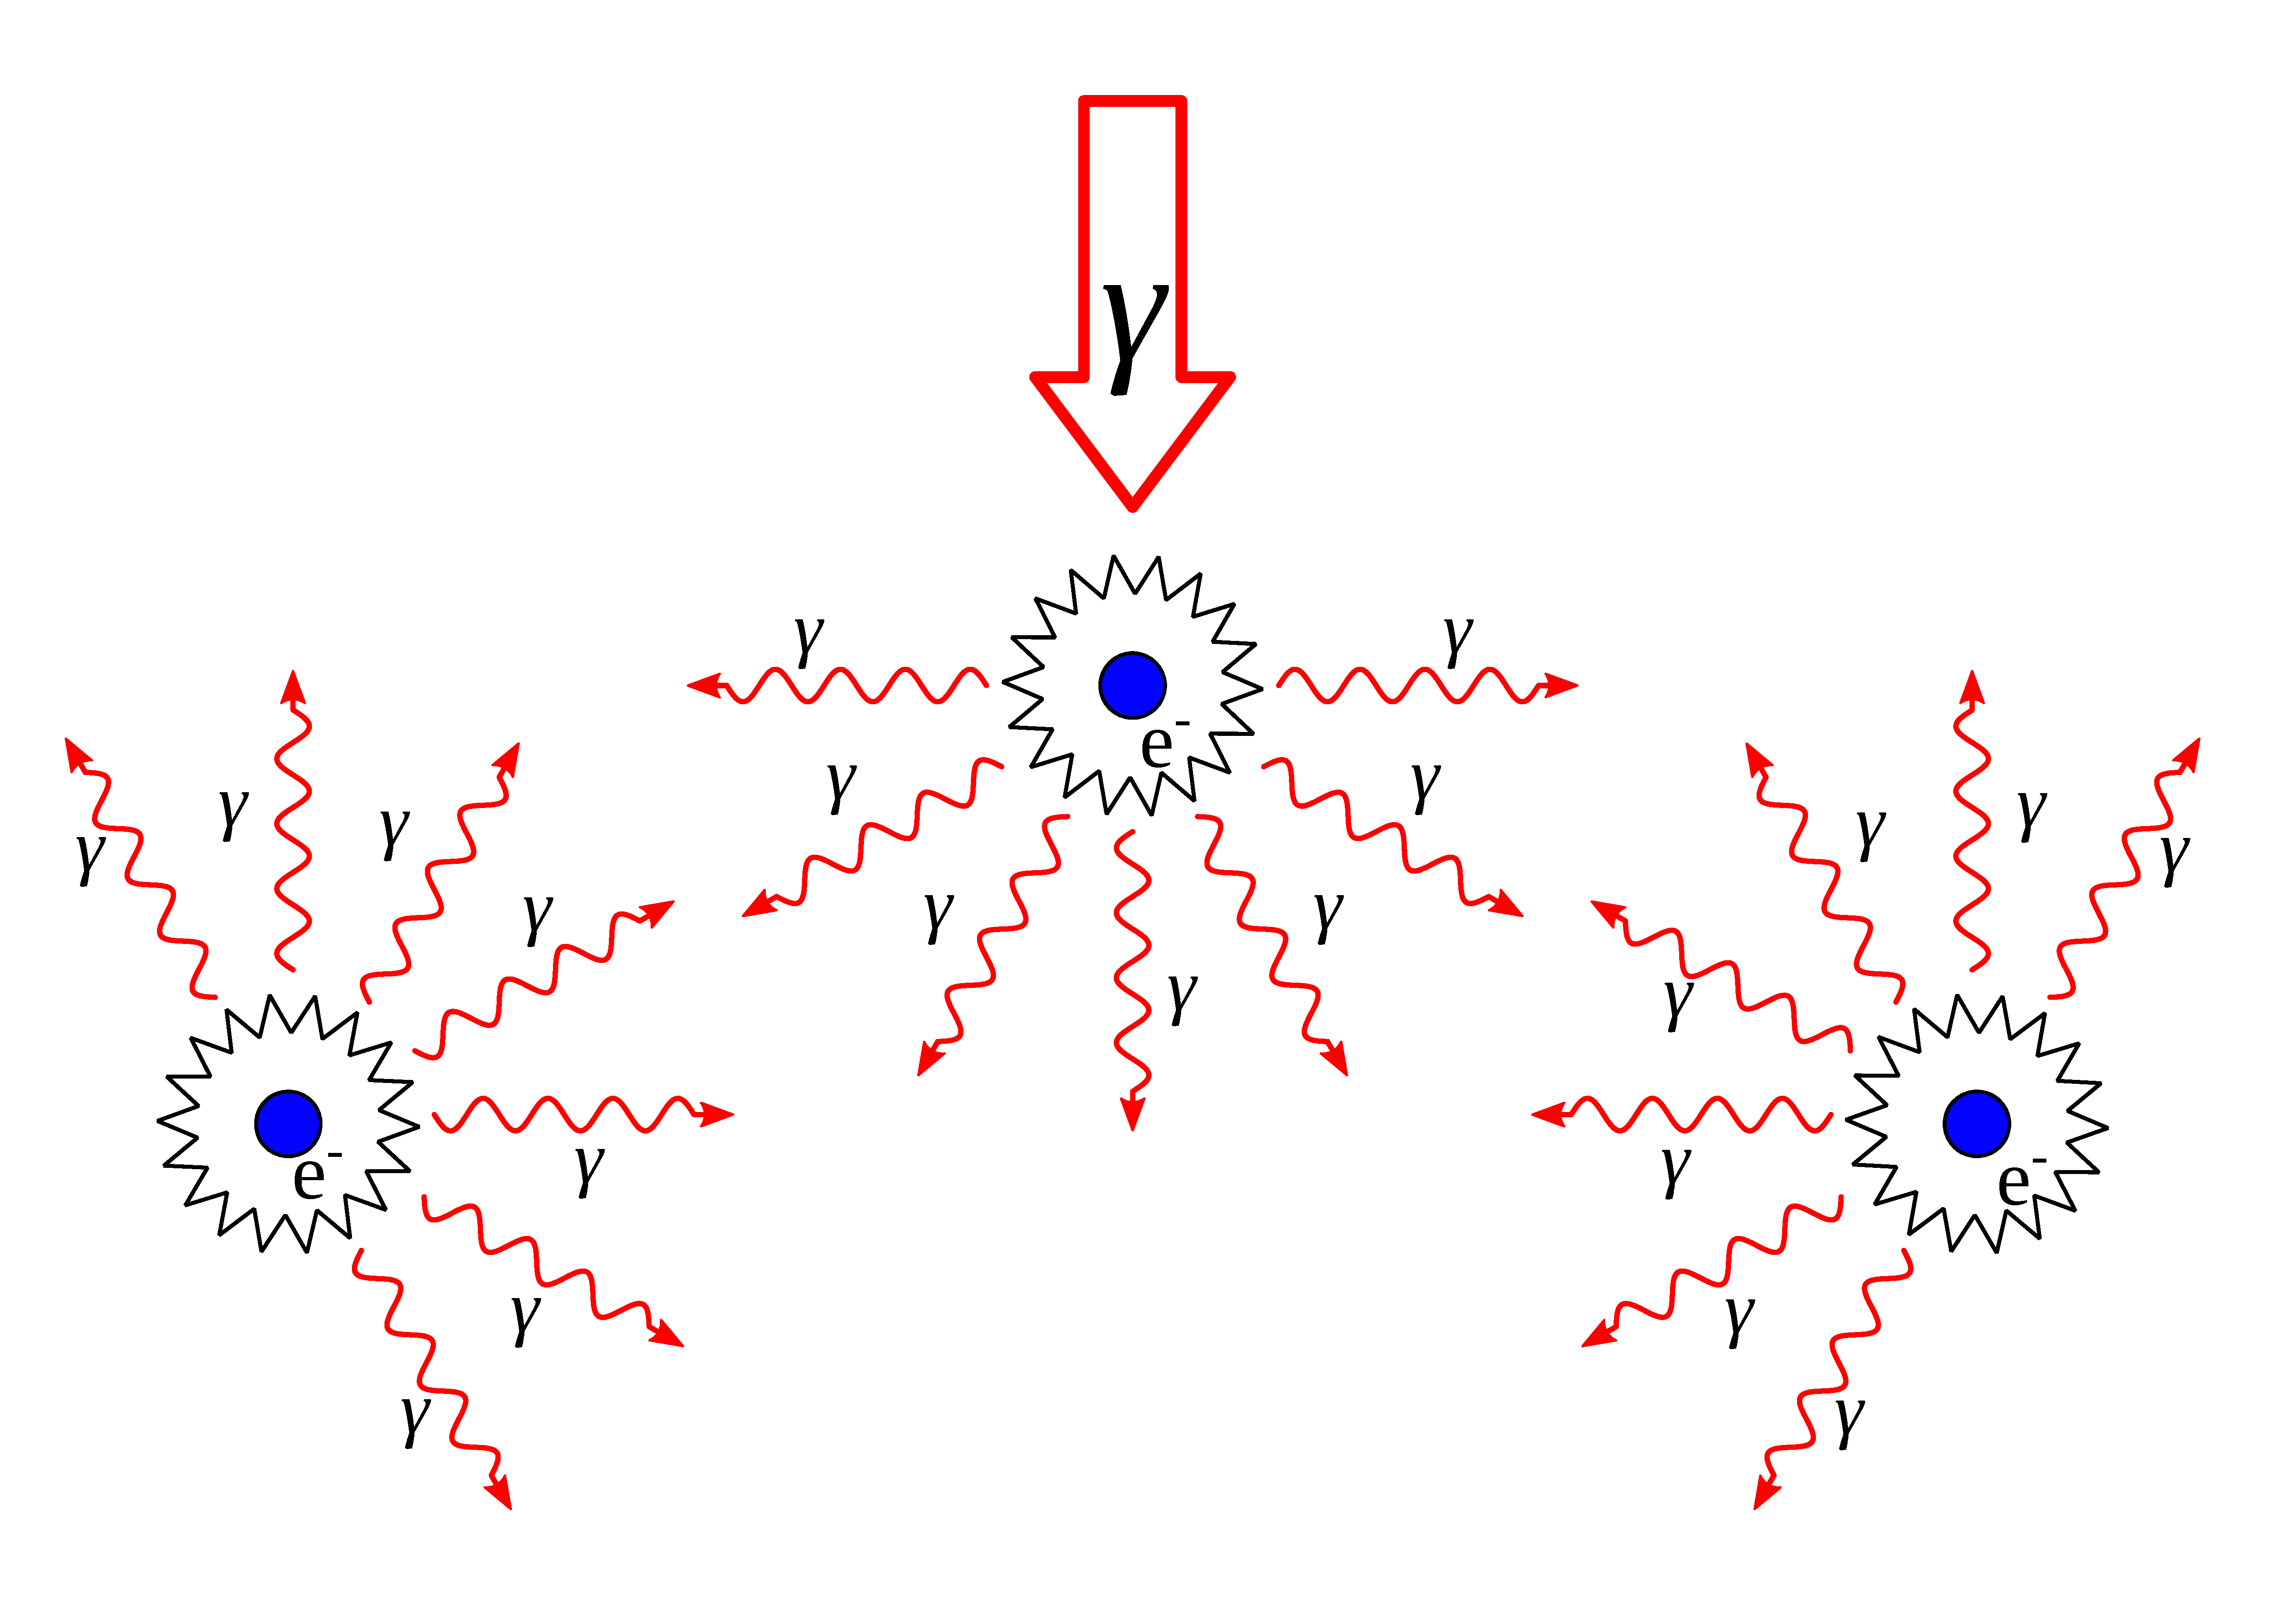
\includegraphics[scale=.15]{thunderstorm/rltge/draw.pdf}}
    \end{overpic}
    \caption{
        Processes occurring in the RL-TGE model: gamma quanta run local acceleration processes in different parts of the cloud with a multidirectional electric field.
    }
    \label{fig:rl}
\end{figure}


\begin{figure}[t]
    \begin{center}
        \begin{minipage}[h]{0.49\linewidth}
            \center{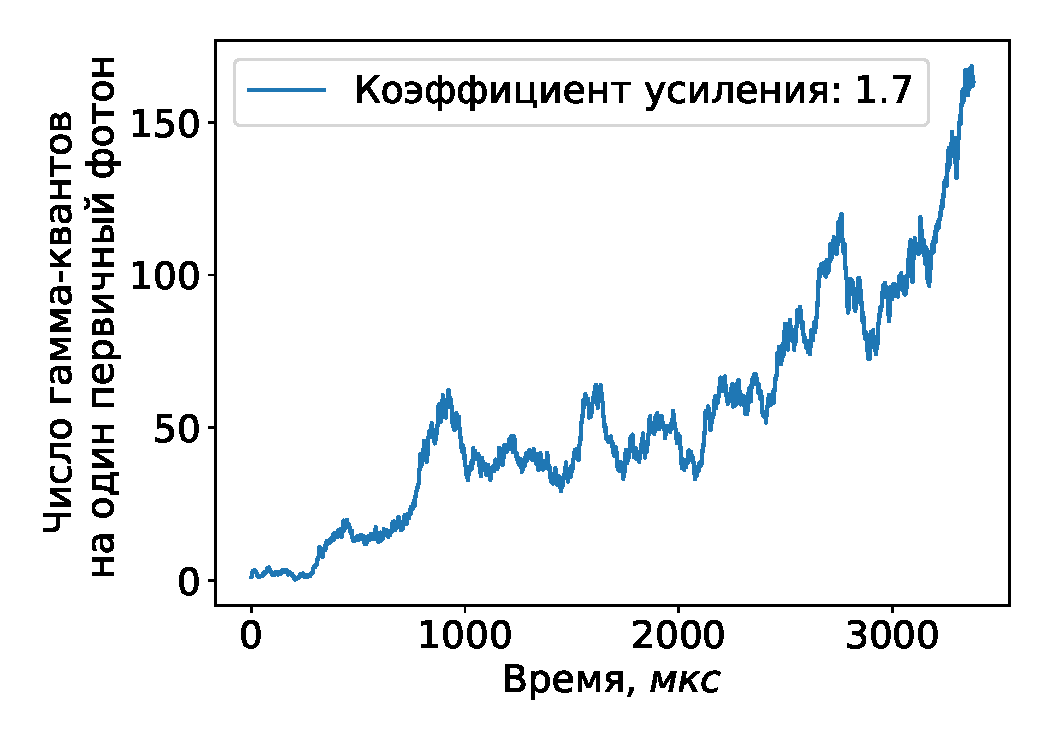
\includegraphics[width=\linewidth]{thunderstorm/RL_proofTGE.pdf} \\ а)}
        \end{minipage}
        \hfill
        \begin{minipage}[h]{0.49\linewidth}
            \center{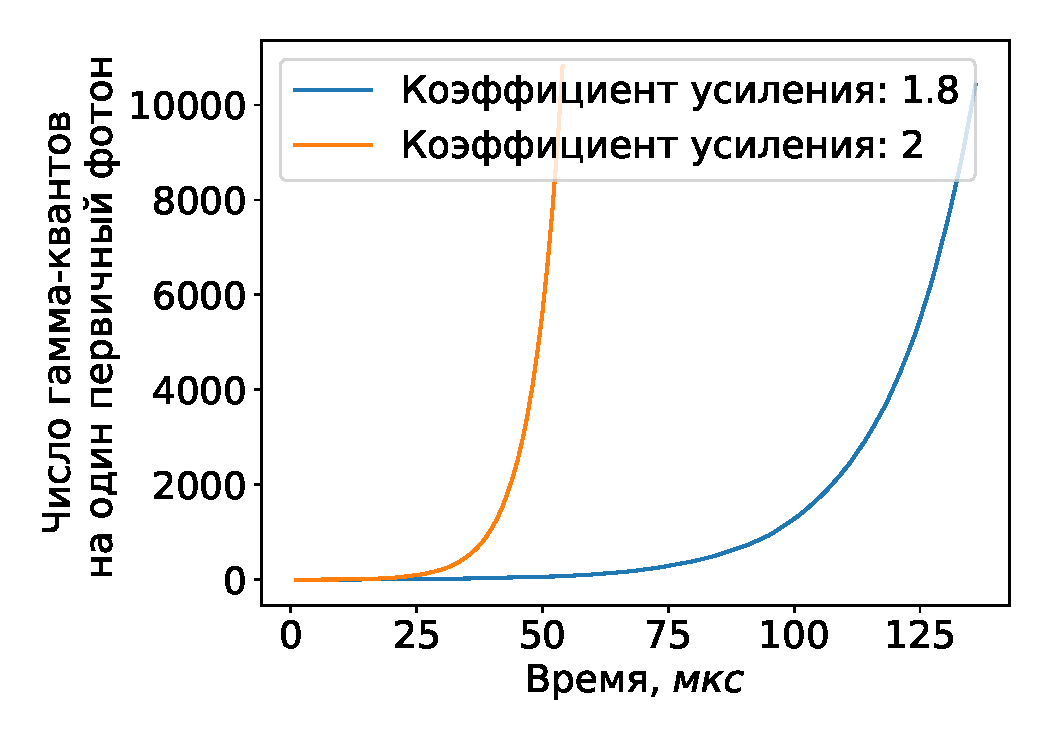
\includegraphics[width=\linewidth]{thunderstorm/RL_proofTGF.pdf}   \\ б)}
        \end{minipage}
        \caption{а) TGE-подобное нарастание. б) TGF-подобное нарастание.}
    \end{center}
    \label{thunder:rl_1}
\end{figure}


\begin{figure}[t]
    \begin{center}
        \begin{minipage}[h]{0.49\linewidth}
            \center{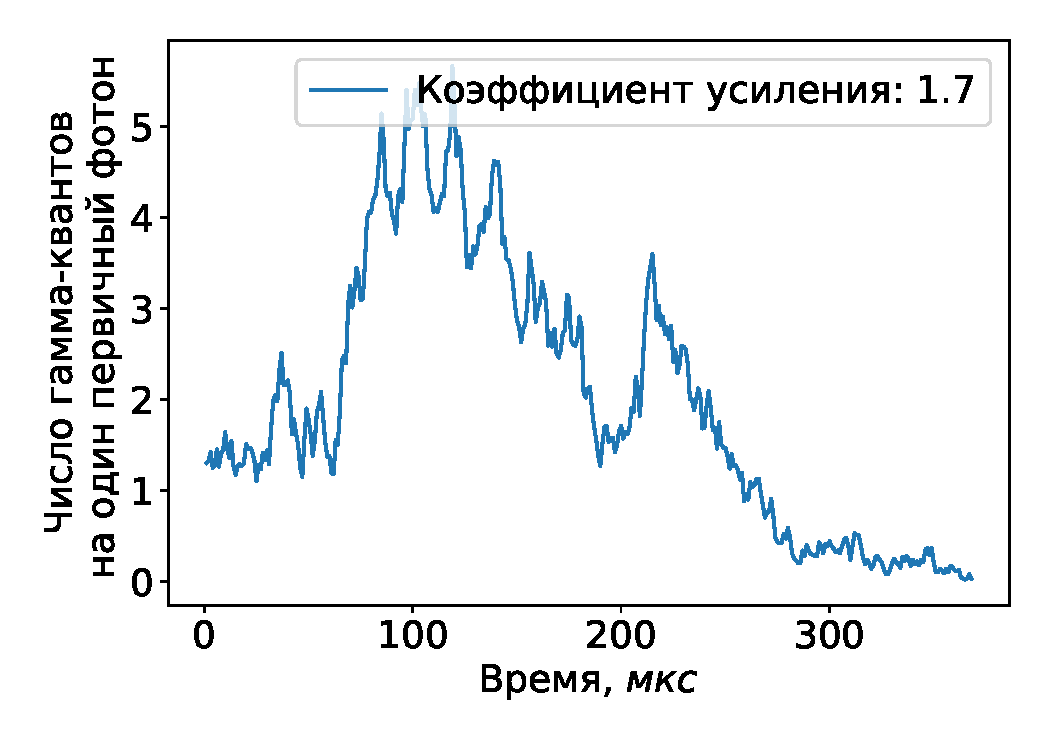
\includegraphics[width=\linewidth]{thunderstorm/RL_Extinction.pdf} \\ а)}
        \end{minipage}
        \hfill
        \begin{minipage}[h]{0.49\linewidth}
            \center{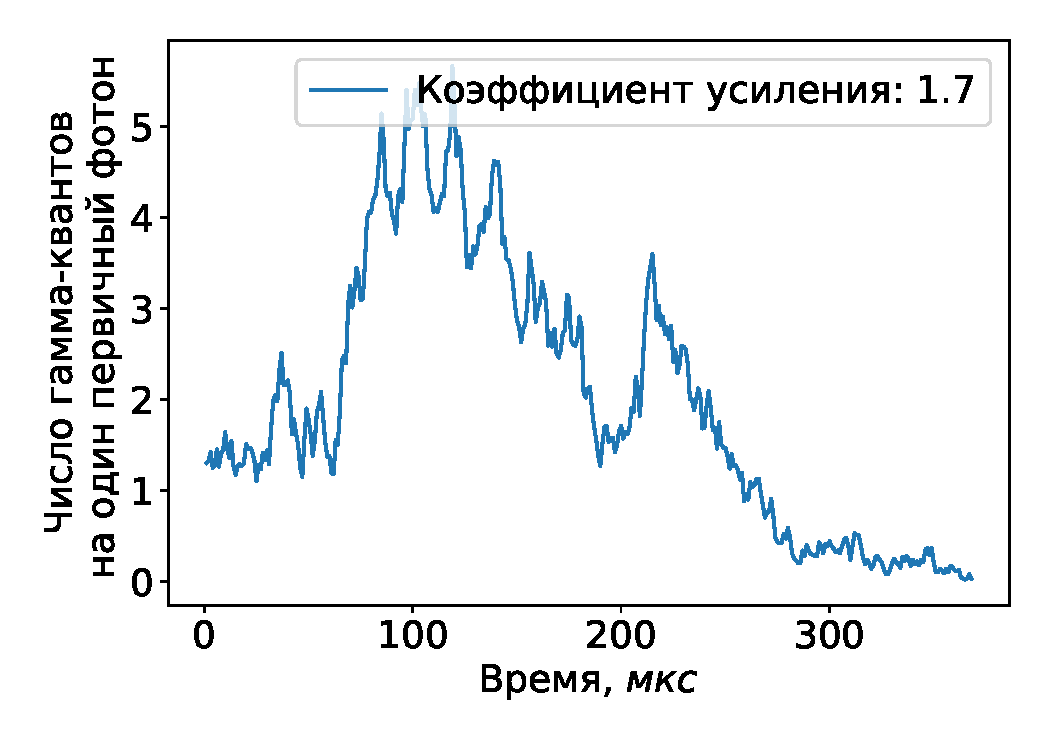
\includegraphics[width=\linewidth]{thunderstorm/RL_Extinction.pdf}   \\ б)}
        \end{minipage}
        \caption{а) Затухание лавины. б) placeholder.}
    \end{center}
    \label{thunder:rl_2}
\end{figure}

\clearpage